\documentclass[11pt,a4paper,notitlepage]{report}
\usepackage[utf8]{inputenc}
\usepackage{amsmath}
\usepackage{amsfonts}
\usepackage{amssymb}
\usepackage{graphicx}
\author{160007345}
\title{Rust Implementation of the ANSI E1.31-2018 sACN Protocol}

\setcounter{secnumdepth}{0}

\begin{document}
	\maketitle
	\section{Rough notes}
	Title page
	Containing the title of the project, the names of the
	student(s), "University of St Andrews" and the date of
	submission. You may add the name of your supervisor
	if you wish.
	
	\section{Abstract}
	Abstract Outline of the project using at most 250 words.
	
	The project expands on an existing implementation \cite{ORIGNIAL_IMPL} of the streaming architecture for control networks (sACN) protocol \cite{ANSI_E1.31} in rust with the aim to make a fully compliant library that allows sending and receiving DMX payload data without having to handle E1.31 specifics directly. This library is made to support Ipv4, Ipv6, unix and windows and is tested to show compliance with the protocol.
	
	\section{Declaration}
	Declaration
	"I declare that the material submitted for
	assessment is my own work except where credit is
	explicitly given to others by citation or
	acknowledgement. This work was performed during
	the current academic year except where otherwise
	stated.
	"The main text of this project report is NN,NNN
	words long, including project specification and plan.
	"In submitting this project report to the University of
	St Andrews, I give permission for it to be made
	available for use in accordance with the regulations of the University Library. I also give permission for
	the title and abstract to be published and for copies of the report to be made and supplied at cost to any bonafide library or research worker, and to be made
	available on the World Wide Web. I retain the
	copyright in this work."
	
	If there is a strong case for the protection of
	confidential data, the parts of the declaration giving
	permission for its use and publication may be omitted
	by prior permission of the Honours Coordinator.
	
	\section{Contents Page}
	\tableofcontents
	
	\section{Introduction}
		Introduction
		
	The goal of this project was to create a rust library for sending and receiving sACN data that is fully compliant with the protocol specification as defined in ANSI E1.31-2018 \cite{ANSI_E1.31}. This project is based on an existing but incomplete implementation of the protocol \cite{ORIGNIAL_IMPL} which was then expanded upon.\\
	
	The following list of objectives
	\begin{list}{}{}
		\item
	\end{list}
	
	Describe the problem you set out to solve and the
	extent of your success in solving it. You should include
	the aims and objectives of the project in order of
	importance and try to outline key aspects of your
	project for the reader to look for in the rest of your
	report.
	
	\section{Context Survey}
	Context survey
	Surveying the context, the background literature and
	any recent work with similar aims. The context survey
	describes the work already done in this area, either as
	described in textbooks, research papers, or in publicly
	available software. You may also describe potentially
	useful tools and technologies here but do not go into
	project-specific decisions.
	\subsection{DMX, SACN and ACN}
	\subsection{Other protocols}
	
	\section{Requirement specification}
	Requirements
	specification
	Capturing the properties the software solution must
	have in the form of requirements specification. You
	may wish to specify different types of requirements and
	given them priorities if applicable.
	
	\section{Software Engineering Process}
		Software
	engineering
	process
	The development approach taken and justification for
	its adoption.

	A waterfall based process model was used for the development of the program. In the waterfall
	method there are several distinct phases of the project as shown in figure: \ref{waterfall-diag}. This 
	development approach was chosen as it has a very clear structure which allows easy to manage distinct milestones 
	so progress through the project can be more easily tracked. This process method has a number of disadvantages aswell
	with the main one being the inflexibility - if something major needed to change it would be difficult to adapt the project. 
	As this project is based on a clearly defined specification provided by the protocal specification and the domains were 
	clearly defined at the start it means that this inflexibility isn't a major issue and so therefore choosing the waterfall 
	method for its advantages makes sense. 
	
	\begin{figure}
		\label{waterfall-diag}
		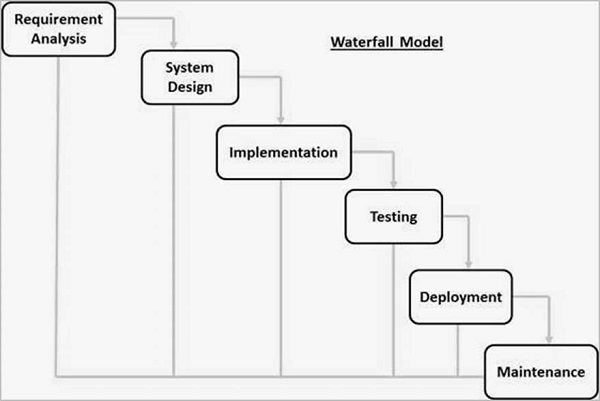
\includegraphics[width=\textwidth]{sdlc_waterfall_model.jpg}
		\caption{A diagram showing the waterfall development process, [\cite{waterfall-diagram}]}
	\end{figure}

	\paragraph*{}
	The waterfall model can be clearly seen throughout the development of the program. The first phase of 'requirement analysis'
	is the protocol specification itself as it clearly lays out the goals of the protocol and what it is required to do. On top of this
	there is the project goals which were defined around the protocol specifically for how much of the protocol this specification should
	implement for example universe-syncronisation, IPv4/IPv6 support, Unix/Windows support etc. When take together this gives a clear list of
	requirements as so allows moving onto the 'system design' phase.

	\paragraph*{}
	The system design phase is where the requirements are turned into a technical plan for how they will be implemented. Alot of this also comes from
	the protocol specification itself as it describes how each bit of a compliant implementation should behave and so therefore the design can be based
	of this.

	\paragraph*{}
	The 'implementation' phase was done 

	One of the requirements
	of the project that was defined was that the implementation should be in rust. This combined with the existing base
	incomplete implementation that was used meant that the general system design was built around this. In general the system
	was designed around there being distinct receivers and senders with communication being mostly one-way. This meant that the two
	different sides could be developed in relative isolation as all their communication must be done in a way that is compliant with the
	protocol which provides the interface between them.

	\paragraph*{}
	The 'testing' phase is the combining of the various bits of the implementation. This is marked by the passing of the various intergration tests
	where the sender and the receiver were passing information back and forth. Also part of this phase is the overall compliance tests which are detailed
	later which show that the implementation of the protocol as a whole conforms to the design and requirements.

	\paragraph*{}
	Once the testing phase has finished the implementation can move onto the 'deployment' phase. In an industry project this would mean 
	distributing the implementation to users and then later moving to the maintenance stage to fix issues or improve various parts of the project
	as opportunities or problems are reported. Within this project the deployment took the form of the development of 2 small programs, one which transmits data 
	specified by the user in the form of various dynamic patterns and a receiver which logs all received input. Theses programs followed a waterfall development
	methodolgy as described later. These programs were then used with various other sACN devices in a real-world environment to show real usage/deployment of
	the protocol. Issues that are discovered at this point can then be fixed through patches which represent the 'maintenance' phase of the program.
	
	\paragraph*{}
	Reflection on the methonolody used
	In general the approach used worked well for the project as it fit the natural development stratergy meaning there weren't any points where the development felt
	like it was 'fighting' the approach chosen. There were a few potential problems that were identified however. One of these was that the model forced rigid time 
	constraints. This is because if too long is spent on any one stage all the subsequent stages would suffer. This was taken as a fairly minor issue for this project 
	because the constraints of fixed submissions deadlines already meant that there some rigid time constraints in place. 

	\ref{waterfall-diagram}
	https://www.tutorialspoint.com/sdlc/sdlc\_waterfall\_model.htm (01/01/2020)
	
	\section{Ethics}
	Ethics
	Any ethical considerations for the project. You should
	scan the signed ethical approval document, and include
	it as an appendix.
	
	\section{Design}
	Design
	Indicating the structure of the system, with particular
	focus on main ideas of the design, unusual design
	features, etc.
	\subsection{ANSI E1.31-2018}
	\subsection{Critique of the protocol}
	\section{Implementation}
	Implementation
	How the implementation was done and tested, with
	particular focus on important / novel algorithms
	and/or data structures, unusual implementation
	decisions, novel user interface features, etc.
	
	\subsection{Implementation dependent specifics}
	
	\section{Evaluation and Critical Appraisal}
	Evaluation and
	critical
	appraisal
	You should evaluate your own work with respect to
	your original objectives. You should also critically
	evaluate your work with respect to related work done
	by others. You should compare and contrast the project
	to similar work in the public domain, for example as
	written about in published papers, or as distributed in
	software available to you.
	
	\section{Conclusions}
	Conclusions
	You should summarise your project, emphasising your
	key achievements and significant drawbacks to your
	work, and discuss future directions your work could be
	taken in.
	
	\section{Appendices}
	The appendices to your report will normally be as follows.
	Testing
	summary
	This should describe the steps taken to debug, test,
	verify or otherwise confirm the correctness of the
	various modules and their combination.
	
	\section{Testing}
	\subsection{Automated Testing}
	\subsection{Real-world Testing}
	
	\section{User Manual}
	User manual Instructions on installing, executing and using the
	system where appropriate.
	
	\section{Other Appendices}
	Other
	appendices
	If appropriate, you may include other material in
	appendices which are not suitable for inclusion in the
	main body of your report, such as the ethical approval
	document.
	You should not include software listings in your project report, unless it is
	appropriate to discuss small sections in the main body of your report. Instead,
	you will submit via MMS your code and associated material such as JavaDoc
	documentation and detailed UML diagrams
	
	\begin{thebibliography}{9}
		\bibitem{ANSI_E1.17}
		ANSI E1.17 - 2015 Entertainment Technology?Architecture for Control Networks
		\bibitem{ORIGNIAL_IMPL}
		https://github.com/lschmierer/sacn (September 2019)
		\bibitem{ANSI_E1.31}
		ANSI E1.31 ? 2018 Entertainment Technology Lightweight streaming protocol for transport of DMX512 using ACN
		\bibitem{DMX_INFO}
		https://www.element14.com/community/groups/open-source-hardware/blog/2017/08/24/dmx-explained-dmx512-and-rs-485-protocol-detail-for-lighting-applications (17/09/2019)
		\bibitem{C_IMPL}
		https://github.com/hhromic/libe131 (17/09/2019)
		\bibitem{RUST_LANG}
		https://www.rust-lang.org/ (17/09/2019)
		\bibitem{ArtNet}
		http://artisticlicence.com/WebSiteMaster/User\%20Guides/art-net.pdf (17/09/2019)
		
		
	\end{thebibliography}
	
\end{document}